\chapter{Integrale}
\section{Einführung}
Der Hauptunterschied zwischen einem bestimmten und einem unbestimmten Integral ist die Existenz (bestimmtes Integral) bzw. das Fehlen
(unbestimmtes Integral) der Integrationsgrenzen.\\
Bei einem bestimmten Integral ist die Lösung ein Flächeinhalt, also ein einfacher Zahlenwert.\\
Bei einem unbestimmten Integral erhält man als Lösung eine Funktion, eine sogenannte Stammfunktion.\\


\section{Bestimmte Integrale}
\begin{Definition}
  Wenn Integrationsgrenzen angegeben werden, handelt es sich um ein bestimmtes Integral:
  \begin{align*}
    \int_{a}^{b} f(x)dx & = \lim\limits_{n \rightarrow \infty} U_n = \lim\limits_{n \rightarrow \infty} s_n\\
                        & = \lim\limits_{n \rightarrow \infty} O_n = \lim\limits_{n \rightarrow \infty} S_n\\
                        & = \lim\limits_{n \rightarrow \infty} \dfrac{b-a}{n}\sum\limits_{k=1}^{n}f\left(\dfrac{b-a}{n}\cdot k\right)
  \end{align*}
  $S_n$ und $O_n$ bezeichnen die Obersumme, wohingegen $s_n$ und $U_n$ die Untersumme bezeichnen.
\end{Definition}

\definecolor{lightblu}{rgb}{0,0,0.3}
\definecolor{lightre}{rgb}{0.3,0,0}
\begin{tikzpicture}
    \draw[->,line width=0.8pt] (-5.5,0) -- (5.5,0) node[below] {$x_1$};
    \draw[->,line width=0.8pt] (0,-5.5) -- (0,5.5) node[right] {$x_2$};
    \foreach  \x in {-5,...,-1,1,2,...,5}
        \draw[line width=0.8pt] (\x,0.1) -- (\x,-0.1) node[below] {\x};
    \foreach  \x in {-5,...,-1,1,2,...,5}
        \draw[line width=0.8pt] (-0.1,\x) -- (0.1,\x) node[right] {\x};
    \draw (-0.3,-0.3) node {$O$};
    \draw[gray,very thin] (-5,-5) grid (5,5);
    \draw[line width=1.5pt,color=red] (-5,2) ..controls(-2,-4) ..(0,0);
    \draw[line width=1.5pt,color=red] (0,0) ..controls(2,4) ..(5,5);
    \draw[line width=0.8pt,fill=lightblu,fill opacity=0.2] (0.5,0) -- (0.5,2.4) -- (1.25,2.4) -- (1.25,0) -- cycle;
    \draw[line width=0.8pt,fill=lightblu,fill opacity=0.2] (1.25,0) -- (1.25,3.5) -- (2,3.5) -- (2,0) -- cycle;
    \draw[line width=0.8pt,fill=lightblu,fill opacity=0.2] (2,0) -- (2,4.1) -- (2.75,4.1) -- (2.75,0) -- cycle;
    \draw[line width=0.8pt,fill=lightblu,fill opacity=0.2] (2.75,0) -- (2.75,4.5) -- (3.5,4.5) -- (3.5,0) -- cycle;
    \draw[line width=0.8pt,fill=lightblu,fill opacity=0.2] (0.5,0) -- (0.5,1) -- (1.25,1) -- (1.25,0) -- cycle;
    \draw[line width=0.8pt,fill=lightblu,fill opacity=0.2] (1.25,0) -- (1.25,2.4) -- (2,2.4) -- (2,0) -- cycle;
    \draw[line width=0.8pt,fill=lightblu,fill opacity=0.2] (2,0) -- (2,3.5) -- (2.75,3.5) -- (2.75,0) -- cycle;
    \draw[line width=0.8pt,fill=lightblu,fill opacity=0.2] (2.75,0) -- (2.75,4.1) -- (3.5,4.1) -- (3.5,0) -- cycle;
    \draw[line width=1.2pt,color=orange] (0.5,1) -- (0.5,0) node[below] {a};
    \draw[line width=1.2pt,color=orange] (3.5,4.5) -- (3.5,0) node[below] {b};
    \draw (1.5,3.8) node {$O_n$};
    \draw (2.375,2.5) node {$U_n$};
    \draw[->,line width=0.8pt] (1.5,-7) -- (12.5,-7) node[below] {$x_1$};
    \draw[->,line width=0.8pt] (7,-12.5) -- (7,-1.5) node[right] {$x_2$};
    \foreach  \x in {2,...,6,8,9,...,12}
        \draw[line width=0.8pt] (\x,-6.9) -- (\x,-7.1);
    \draw (2,-7.1) node[below] {-5};
    \draw (3,-7.1) node[below] {-4};
    \draw (4,-7.1) node[below] {-3};
    \draw (5,-7.1) node[below] {-2};
    \draw (6,-7.1) node[below] {-1};
    \draw (8,-7.1) node[below] {1};
    \draw (9,-7.1) node[below] {2};
    \draw (10,-7.1) node[below] {3};
    \draw (11,-7.1) node[below] {4};
    \draw (12,-7.1) node[below] {5};
    \foreach  \x in {-12,...,-8,-6,-5,...,-2}
        \draw[line width=0.8pt] (6.9,\x) -- (7.1,\x);
    \draw (7.1,-12)[right] node{-5}:
    \draw (7.1,-11)[right] node{-4}:
    \draw (7.1,-10)[right] node{-3}:
    \draw (7.1,-9)[right] node{-2}:
    \draw (7.1,-8)[right] node{-1}:
    \draw (7.1,-6)[right] node{1}:
    \draw (7.1,-5)[right] node{2}:
    \draw (7.1,-4)[right] node{3}:
    \draw (7.1,-3)[right] node{4}:
    \draw (7.1,-2)[right] node{5}:
    \draw (6.7,-7.3) node {$O$};
    \draw[gray,very thin] (2,-12) grid (12,-2);
    \draw[line width=1.5pt,color=blue] (2,-9) ..controls(5,-3) ..(7,-4);
    \draw[line width=1.5pt,color=blue] (7,-4) ..controls(10,-5) ..(12,-9);
    \draw[line width=0.8pt,fill=lightre,fill opacity=0.2] (7.5,-7) -- (7.5,-4.2) -- (8.25,-4.2) -- (8.25,-7) -- cycle;
    \draw[line width=0.8pt,fill=lightre,fill opacity=0.2] (8.25,-7) -- (8.25,-4.4) -- (9,-4.4) -- (9,-7) -- cycle;
    \draw[line width=0.8pt,fill=lightre,fill opacity=0.2] (9,-7) -- (9,-4.75) -- (9.75,-4.75) -- (9.75,-7) -- cycle;
    \draw[line width=0.8pt,fill=lightre,fill opacity=0.2] (9.75,-7) -- (9.75,-5.25) -- (10.5,-5.25) -- (10.5,-7) -- cycle;
    \draw[line width=0.8pt,fill=lightre,fill opacity=0.2] (7.5,-7) -- (7.5,-4.4) -- (8.25,-4.4) -- (8.25,-7) -- cycle;
    \draw[line width=0.8pt,fill=lightre,fill opacity=0.2] (8.25,-7) -- (8.25,-4.75) -- (9,-4.75) -- (9,-7) -- cycle;
    \draw[line width=0.8pt,fill=lightre,fill opacity=0.2] (9,-7) -- (9,-5.25) -- (9.75,-5.25) -- (9.75,-7) -- cycle;
    \draw[line width=0.8pt,fill=lightre,fill opacity=0.2] (9.75,-7) -- (9.75,-6.2) -- (10.5,-6.2) -- (10.5,-7) -- cycle;
    \draw[line width=1.2pt,color=orange] (7.5,-4.2) -- (7.5,0-7) node[below] {a};
    \draw[line width=1.2pt,color=orange] (10.5,-6.2) -- (10.5,-7) node[below] {b};
    \draw (9.5,-4.4) node {$O_n$};
    \draw (8.625,-5.6) node {$U_n$};
    \draw[line width=2pt] (-5,-12) -- (12,5);
\end{tikzpicture}

\begin{Bemerkung}
  $a$ und $b$ bezeichnen jeweils die untere und obere Grenze des zu berechnenden Integrals. Sie bezeichnen anschaulich die $x$-Werte, zwischen denen die Fläche berechnet wird.
\end{Bemerkung}
\begin{Bemerkung}
  Im allgemeinen Fall muss der Integrand $f(x)$ im Intervall $[a;b]$ stetig sein, damit das Integral bestimmt ist.
\end{Bemerkung}

\section{Stammfunktionen und der Hauptsatz der Differential- und Integralrechnung}
\begin{Definition}
  Eine Funktion $F$ heißt Stammfunktion der Funktion $f$, wenn $F'(x)=f(x)$
  gilt.\\
  Ist $F$ irgendeine Stammfunktion von $f$, dann ist auch $F(x)+C$ (mit
  konstantem $C$) eine Stammfunktion, denn beim Ableiten fällt $C$ als
  konstanter Summand weg. Jede Funktion hat also unendlich viele
  Stammfunktionen, die sich aber nur um einen konstanten Summanden
  unterscheiden.
\end{Definition}
\begin{Bemerkung}
  Man beobachtet hier eine Erwiterung der NEW-Regel (siehe \ref{NEW-Regel}, NEW-Regel):\\\\
  \begin{minipage}[b]{0.2\linewidth}
    N $=$ Nullstellen\\
    E $=$ Extremstellen\\
    W $=$ Wendestellen
  \end{minipage}
  \hfill \vline \hfill
  \begin{minipage}[b]{0.4\linewidth}
    \begin{array}{rcccccl}
    F &   N & E & W & & \\
    f & \qquad \qquad& N & E & W & & \\
    f' & \qquad \qquad && N & E & W & \\
    \end{array}
  \end{minipage}
\end{Bemerkung}
\subsection{Sätze über Integrale}
Layout muss noch angepasst werden\\
\begin{Theorem}
  \begin{minipage}{0.6\textwidth}
    \begin{align*}
      \int_a^b f(x)dx &= -\int_b^a f(x)dx\\\\
      \int_a^b (f(x)+g(x))dx &= \int_a^b f(x)dx + \int_a^b g(x)dx\\\\
      \int_a^b r*f(x)dx &= r*\int_a^b f(x)dx\\\\
      \int_a^b f(x)dx + \int_b^c f(x)dx &= \int_a^c f(x)dx
    \end{align*}
  \end{minipage}
  \begin{minipage}{0.4\textwidth}
    \\\\\\
    Invertieren der Intergrationsgrenzen\\\\\\\\
    Summenregel\\\\\\\\
    Linearität\\\\\\\\
    Abschnittweise Integration
  \end{minipage}

\end{Theorem}
Invertieren der Intergrationsgrenzen:
\begin{Beweis}
  $$\int_a^b f(x)dx = F(b)-F(a) = -(F(a)-F(b)) = -\int_b^a f(x)dx$$
\end{Beweis}
\\
Summenregel:
\begin{Beweis}
  $$\int_a^b f(x)+g(x)dx = [F(x)+G(x)]_a^b = F(b)+G(b)-(F(a)+G(b)) = F(b)-F(a)+G(b)-G(b) $$$$= \int_a^b f(x)dx+\int_a^b g(x)dx$$
\end{Beweis}
\\
Linearität:
\begin{Beweis}
  $$\int_a^b r*f(x)dx = [r*F(x)]_a^b = r*F(b)-r*F(a) = r*(F(a)-F(b)) = r*\int_a^b f(x)dx$$
\end{Beweis}
\\
Abschnittweise Integration:
\begin{Beweis}
  $$\int_a^b f(x)dx+ \int_b^c f(x)dx = F(a)-F(b)-(F(b)-F(c)) = F(c)-F(a) = \int_a^c f(x)dx$$
\end{Beweis}

\begin{Theorem}
  Sei eine in $[a;b]$ stetige Funktion $f$. Wenn für $m,M \in \R$ gilt: $m\leq f(t) \leq M \; \forall t \in [a;b]$, dann gilt:
  $$m(b-a) \leq \int_a^b f(t)dt \leq M(b-a)$$
\end{Theorem}
\begin{Beweis}
  Es reicht, $m \leq f(t) \leq M$ als Ungleichung zwischen $a$ und $b$ zu integrieren.
\end{Beweis}

\begin{center}
    \definecolor{lightblu}{rgb}{0,0,0.3}
    \definecolor{blu}{rgb}{0,0.3,0.3}
    \definecolor{lightgree}{rgb}{0,0.3,0}
    \definecolor{gree}{rgb}{0.1,0.3,0}
    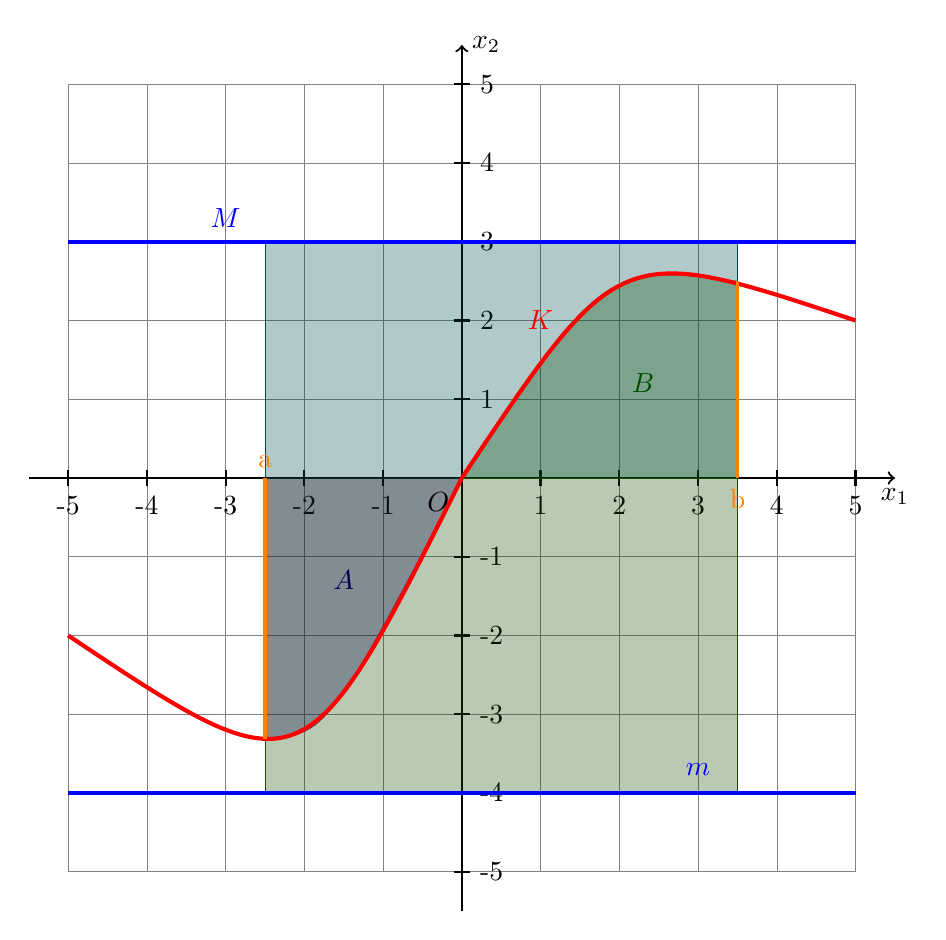
\begin{tikzpicture}
        \draw[gray,very thin] (-5,-5) grid (5,5);

        \draw[->,line width=0.8pt] (-5.5,0) -- (5.5,0) node[below] {$x_1$};
        \draw[->,line width=0.8pt] (0,-5.5) -- (0,5.5) node[right] {$x_2$};
        \foreach  \x in {-5,...,-1,1,2,...,5}
            \draw[line width=0.8pt] (\x,0.1) -- (\x,-0.1) node[below] {\x};
        \foreach  \x in {-5,...,-1,1,2,...,5}
            \draw[line width=0.8pt] (-0.1,\x) -- (0.1,\x) node[right] {\x};

        \draw[line width=0.1pt,color=blu,fill=blu,fill opacity=0.3] (-2.5,0) -- (-2.5,3) -- (3.5,3) -- (3.5,0) -- cycle;
        \draw[line width=0.1pt,color=gree,fill=gree,fill opacity=0.3] (-2.5,0) -- (-2.5,-4) -- (3.5,-4) -- (3.5,0) -- cycle;
        \draw[line width=0.1pt,color=lightblu,fill=lightblu,fill opacity=0.3] (-2.5,0) -- (-2.5,-3.32) ..controls(-1.71,-3.25) ..(0,0) -- cycle;
        \draw[line width=0.1pt,color=lightgree,fill=lightgree,fill opacity=0.3] (0,0) ..controls(1.8,2.7) ..(3.5,2.5) -- (3.5,0) -- cycle;

        \draw[line width=1.5pt,color=red] (-5,-2) ..controls(-2,-4) ..(0,0);
        \draw[line width=1.5pt,color=red] (0,0) ..controls(2,3) ..(5,2);

        \draw[line width=1.5pt,color=blue] (-5,3) -- (5,3);
        \draw[line width=1.5pt,color=blue] (-5,-4) -- (5,-4);

        \draw[line width=1.2pt,color=orange] (-2.5,-3.32) -- (-2.5,0) node[above] {a};
        \draw[line width=1.2pt,color=orange] (3.5,2.5) -- (3.5,0) node[below] {b};

        \draw (-0.3,-0.3) node {$O$};
        \draw[line width=0.8pt,color=lightblu] (-1.5,-1.3) node {$A$};
        \draw[line width=0.8pt,color=lightgree] (2.3,1.2) node {$B$};

        \draw[line width=0.8pt,color=red] (1,2) node {$K$};
        \draw[line width=0.8pt,color=blue] (-3,3.3) node {$M$};
        \draw[line width=0.8pt,color=blue] (3,-3.7) node {$m$};
    \end{tikzpicture}
\end{center}

\begin{Bemerkung}
  Eine Konsequenz davon ist, dass falls $|f(t)|\leq M \; \forall t \in [a;b]$, dann gilt:
  $$\left|\int_a^b f(t)dt \right| \leq M(|b-a|)$$
\end{Bemerkung}
\subsection{Integrationsregeln}
\subsubsection{Partielle Integration}
\begin{Theorem}
  Seien $u$ und $v$ zwei stetig differenzierbare Funktionen im Intervall $I$ und $u'$
  und $v'$ in I stetig. Dann gilt:
  $$\int u(x)'v(x) dx= u(x)v(x) - \int u(x)v'(x) dx$$
\end{Theorem}
\begin{Beweis}\\
Nachweisen u, v diffbar und u', v' stetig (kommt noch in sauber)\\
\begin{align*}
  &&(u(x)*v(x))' &= u'(x)v(x)+u(x)v'(x)\\
  &\Leftrightarrow & \int (u(x)*v(x))' dx &= \int u'(x)v(x)+\int u(x)v'(x)\\
  &\Leftrightarrow & u(x)*v(x) &= \int u'(x)v(x)+\int u(x)v'(x)\\
  &\Leftrightarrow & \int u(x)v'(x) &= u(x)*v(x)- \int u'(x)v(x)\\
\end{align*}
\end{Beweis}
\begin{Beispiel}
  \begin{align*}
  \int x\sin(x) dx &= \int x(-\cos(x))' dx\\
  &= -x\cos(x) - \int-\cos(x)*1 dx\\
  &= -x\cos(x) + \int\cos(x) dx\\
  &= -x\cos(x) + \sin(x)
\end{align*}
\end{Beispiel}
\subsubsection{Substitution}
Es soll die Stammfunktion von $x(1-x^2)^9$ bestimmt werden. Hier wäre zum
Ableiten die Kettenregel und die Produktregel nötig, beides gibt es aber in
reiner Form beim Integrieren nicht. Man kann aber häufig durch geschickte
Substitution das Integral auf eine Form bringen, für die dann eine
Stammfunktion angegeben werden kann. Der wesentliche Punkt dabei ist, dass
nicht nur $x$ sondern auch $\dD x$ der Substitution unterworfen werden muss.

In diesem Beispiel setzen wir $u=1-x^2$. Dann ist $\dD u=u'(x)\dD x=-2x\dD x$.
Somit ist $\dD x=-\dD u/2x$. Nun geht's los:
\[
\int x(1-x^2)^9\dD x=\int x u^9 \frac{-1}{2x}\dD u
=-\frac{1}{2}\int u^9\dD u=-\frac{1}{20}u^{10}=-\frac{1}{20}(1-x^2)^{10}
\]

Hätten wir hier die Stammfunktion nicht benötigt, sondern nur den Wert eines
bestimmten Integrals, dann hätte man sich die Rücksetzung sparen können, indem
man die Grenzen auf die neue Variable umschreibt:
\[
\int_{x=0}^1 x(1-x^2)^9\dD x=-\frac{1}{2}\int_{u=1}^0u^9\dD u
=-\frac{1}{20}\left[u^{10}\right]_1^0=-\frac{1}{20}(0-1)=\frac{1}{20}
\]

In diesem Beispiel haben wir einen Teilausdruck des Integrals gleich $u$
gesetzt. Im folgenden Beispiel machen wir es anders herum und setzen $x$
gleich einer Funktion von $u$. Es soll die Fläche einer Ellipse berechnet
werden. Für den oberen Ellipsenbogen gilt die Gleichung (Auflösen der
Mittelpunktsform~\eqref{eq:7} nach $y$):
\[
y=\frac{b}{a}\sqrt{a^2-x^2}
\]
Die Fläche unter dem oberen Ellipsenbogen ist die halbe Ellipsenfläche und
berechnet sich so:
\[
A=\int\limits_{x=-a}^a \frac{b}{a}\sqrt{a^2-x^2}\,\dD x=
\int\limits_{u=-\frac{\pi}{2}}^{\frac{\pi}{2}}
\frac{b}{a}\sqrt{a^2-a^2\sin^2u}\,a\cos u\,\dD u=
\int\limits_{-\frac{\pi}{2}}^{\frac{\pi}{2}}ab\cos^2u\,\dD u
\]
Dabei hat man $x=a\sin u$ gesetzt, dann wird $\dD x=a\cos u \dD u$. Nun muss
man nur noch die Stammfunktion von $\cos^2u$ ermitteln. Dazu kann man etwa die
Beziehung $\cos2u=2\cos^2u-1$ heranziehen, also
$\cos^2u=\frac{1}{2}(1+\cos2u)$. Diese hat die Stammfunktion
$\frac{1}{2}(u+\sin u\cos u)$. Damit bekommt man für die Fläche:
\[
A=\frac{ab}{2}\left[u+\sin u\cos u\right]_{-\frac{\pi}{2}}^{+\frac{\pi}{2}}=
\frac{ab}{2}[(\frac{\pi}{2}+0)-(-\frac{\pi}{2}+0)]=\frac{1}{2}\pi a b
\]
Die gesamte Fläche der Ellipse ist doppelt so groß, also $\pi a b$.

\subsubsection{Partialbruchzerlegung}
Die Partialbruchzerlegung ist ein allgemeines Verfahren zur Integration
gebrochen rationaler Funktionen. Es sei gegeben:
\begin{equation}
  \label{eq:68}
  f(x)=\frac{P(x)}{Q(x)}
  =\frac{a_0+a_1x+\dots+a_nx^n}{b_0+b_1x+\dots+b_mx^m}
\end{equation}
Im Falle $m\le n$ führt man zuerst eine Polynomdivision aus, dann bekommt man
eine ganzrationale Funktion und eine gebrochen rationale mit $m>n$, so dass
wir uns für das Weitere auf den Fall $m>n$ beschränken können.

Das Nennerpolynom kann im Komplexen vollständig in Linearfaktoren zerlegt
werden, im Reellen bleiben ggf. quadratische Faktoren übrig, die keine reellen
Nullstellen mehr haben. Seien nun $x_k$ die Nullstellen von $Q(x)$ mit der
Vielfachheit $\nu_k$ dann kann man $Q(x)$ stets auf die folgende Form bringen:
\begin{equation}
  \label{eq:69}
  Q(x)=b_m(x-x_1)^{\nu_1}(x-x_2)^{\nu_2}\dots(x-x_k)^{\nu_k}
  (x^2+\alpha_1x+\beta_1)^{\mu_1}\dots(x^2+\alpha_rx+\beta_r)^{\mu_r}
\end{equation}
Die gebrochen rationale Funktion $f(x)$ lässt sich nun als Summe von
Partialbrüchen schreiben. Dabei gilt:
\begin{enumerate}
\item Jeder Linearfaktor $(x-x_k)$ der Vielfachheit $\nu_k$ trägt zur
  Zerlegung die folgenden Summanden bei:
  \[
  \frac{A_1}{(x-x_k)}+\frac{A_2}{(x-x_k)^2}+\dots
  +\frac{A_{\nu_k}}{(x-x_k)^{\nu_k}}
  \]
\item Jeder quadratische Faktor mit der Vielfachheit $\mu_k$ trägt die
  folgenden Summanden bei:
  \[
  \frac{C_1x+D_1}{(x^2+\alpha x+\beta)}+
  \frac{C_2x+D_2}{(x^2+\alpha x+\beta)^2}+\dots+
  \frac{C_{\mu_k}x+D_{\mu_k}}{(x^2+\alpha x+\beta)^{\mu_k}}
  \]
\end{enumerate}

\noindent Die Linearfaktoren lassen sich sofort integrieren, bei den
quadratischen geht man so vor:
\[
(x^2+\alpha x+\beta)=\bigl(x+\tfrac{\alpha}{2}\bigr)^2+\delta^2
=(\delta y)^2+\delta^2=\delta^2(y^2+1)
\]
Hier hat man quadratisch ergänzt und $\delta\cdot y=x+\frac{\alpha}{2}$
substituiert. Mit dieser Substitution ist
\[
x=\delta y-\frac{\alpha}{2}\qquad y=\frac{x+\frac{\alpha}{2}}{\delta}\qquad
\dD x=\delta\dD y
\]
Nun wird das Integral zu:
\begin{align*}
  \int\frac{Cx+D}{(x^2+\alpha x+\beta)^\mu}\dD x
  &=\frac{1}{\delta^{2\mu-1}}
  \int\frac{C\delta y+D-\frac12C\alpha}{(y^2+1)^\mu}\dD y\\
  &=\frac{C}{\delta^{2\mu-2}}\int\frac{y\dD y}{(y^2+1)^\mu}
  +\frac{D-\frac12C\alpha}{\delta^{2\mu-1}}\int\frac{\dD y}{(y^2+1)^\mu}
\end{align*}
Für das erste der beiden verbleibenden Integrale bekommt man dann
\begin{equation}
  \label{eq:70}
  \int\frac{y\dD y}{(y^2+1)^\mu}=\frac12\int\frac{\dD u}{u^\mu}=
  \begin{cases}
    \dfrac{u^{1-\mu}}{2(1-\mu)}=&\text{für~}\mu=2, 3, \dots\\
    \frac{1}{2}\ln|u|& \text{für~} \mu=1
  \end{cases}
\end{equation}
Hier hat man $u=y^2+1$ gesetzt. Nun muss noch das zweite bestimmt werden.
\[
J_\mu=\int\frac{\dD y}{(y^2+1)^\mu}
\]
Für $\mu=1$ ist es bekannt, $J_1=\arctan y$.

Wir werden eine Rekursionsformel für die $J_\mu$ herleiten. Wir beginnen mit
der Beziehung
\[
J_{\mu+1}=\int\frac{(y^2+1)-y^2}{(y^2+1)^{\mu+1}}\dD y
=J_\mu-\int\frac{y^2}{(y^2+1)^{\mu+1}}\dD y
\]
Nun denken wir uns den zweiten Integranden als $y\cdot$Rest geschrieben und
integrieren partiell:
\[
\int y\cdot\frac{y\dD y}{(y^2+1)^{\mu+1}}=
\frac{-y}{2\mu(y^2+1)^\mu}+\frac{1}{2\mu}\int\frac{\dD y}{(y^2+1)^\mu}=
\frac{-y}{2\mu(y^2+1)^\mu}+\frac{1}{2\mu}\,J_\mu
\]
Setzt man das oben ein, so bekommt man die Rekursionsformel:
\begin{equation}
  \label{eq:71}
  J_{\mu+1}=\left(1-\frac{1}{2\mu}\right)J_\mu+\frac{y}{2\mu(y^2+1)^\mu}
\end{equation}
Insbesondere ist dann (rechne das nach!)
\begin{align*}
  J_1&=\arctan y\\
  J_2&=\frac{1}{2}\arctan y+\frac{y}{2(y^2+1)}\\
  J_3&=\frac38\left(\arctan y+\frac{y}{y^2+1}\right)+\frac{y}{4(y^2+1)^2}\\
  J_4&=\frac{5}{16}\left(\arctan y+\frac{y}{y^2+1}\right)+
       \frac{5}{24}\cdot\frac{y}{(y^2+1)^2}+\frac{y}{6(y^2+1)^3}
\end{align*}
\subsubsection{Integrale von $e$-Funktionen}
\begin{Theorem}
  Für $f(x)=e^{l(x)}$ mit $l(x) = ax+b$ gilt:\\
  $F(x) = \dfrac{1}{a}e^{l(x)}$
\end{Theorem}
\begin{Beweis}
  Not yet... ;((
\end{Beweis}
\subsubsection{Integrale von $ln()$-Funktionen}
\begin{Theorem}
  Für $x \in \R^{+}$ ist $F$ eine Stammfunktion zur Funktion $f(x) = \ln(x)$ mit $F(x) = x \ln(x)-x$
\end{Theorem}
\begin{Beweis}
  Der Beweis erfolgt über partielle Integration und wird dem Schüler als Übung überlassen.
\end{Beweis}
\subsubsection{Integrale von periodischen Funktionen}
\begin{Theorem}
  Für jede auf $\R$ stetige und periodische Funktion $f$ gilt:\\\\
  $\int_a^{a+T} f(x)dx$ ist unabhängig von $a$ und $\int_a^{a+T} f(x)dx = \int_0^{T} f(x)dx$
\end{Theorem}
\begin{Beweis}
  Patience...
\end{Beweis}

\subsection{Merkenswerte Integrale}
\begin{align*}
  \int x^n dx&=\frac{x^{n+1}}{n+1}\\
  \int\sin x dx&= -\cos x\\
  \int\cos x dx&= \sin x\\
  \int\frac{ dx}{\cos^2x}&= \tan x\\
  \int\frac{1}{x} dx&= \ln(|x|)\\
\end{align*}
ln, e^x, usw.

\section{Flächen und Volumen mit Integralen berechnen}
\subsection{Fläche zwischen einer Funktion und der $x_1$-Achse}
\begin{Definition}
  Für die auf dem Intervall $[a;b]$ (also stückweise) stetige Funktion $f$ mit Nullstellen und $x_1,x_2,...,x_n$
  mit $a \leq x_1 \leq x_2 \leq ... \leq x_n \leq b$ ist der Flächeninhalt $A$ zwischen dem Graphen von $f$ und
  der $x_1$-Achse im Intervall $[a;b]$ gegeben durch:
  $$A= \left|{\int_a^{x_1} f(x)dx}\right|+\left|{\int_{x_1}^{x_2} f(x)dx}\right|+...+\left|{\int_{x_{n-1}}^{x_n} f(x)dx}\right|+\left|{\int_{x_n}^b f(x)dx}\right|$$
\end{Definition}
Bildhaft sieht das folgendermaßen aus:\\
\begin{center}
    \definecolor{lightblu}{rgb}{0,0,0.3}
    \definecolor{lightgree}{rgb}{0,0.3,0}
    \begin{tikzpicture}
        \draw[gray,very thin] (-5,-5) grid (5,5);

        \draw[->,line width=0.8pt] (-5.5,0) -- (5.5,0) node[below] {$x_1$};
        \draw[->,line width=0.8pt] (0,-5.5) -- (0,5.5) node[right] {$x_2$};
        \foreach  \x in {-5,...,-1,1,2,...,5}
            \draw[line width=0.8pt] (\x,0.1) -- (\x,-0.1) node[below] {\x};
        \foreach  \x in {-5,...,-1,1,2,...,5}
            \draw[line width=0.8pt] (-0.1,\x) -- (0.1,\x) node[right] {\x};

        \draw[line width=0.1pt,color=lightblu,fill=lightblu,fill opacity=0.3] (-2.5,0) -- (-2.5,-2.5) ..controls(-1.62,-3.072) ..(0,0) -- cycle;
        \draw[line width=0.1pt,color=lightgree,fill=lightgree,fill opacity=0.3] (0,0) ..controls(1.94,3.78) ..(3.5,4.5) -- (3.5,0) -- cycle;

        \draw[line width=1.5pt,color=red] (-5,2) ..controls(-2,-4) ..(0,0);
        \draw[line width=1.5pt,color=red] (0,0) ..controls(2,4) ..(5,5);

        \draw[line width=1.2pt,color=orange] (-2.5,-2.5) -- (-2.5,0) node[above] {a};
        \draw[line width=1.2pt,color=orange] (0,-0.2) node[right] {$x_1$};
        \draw[line width=1.2pt,color=orange] (3.5,4.5) -- (3.5,0) node[below] {b};

        \draw[line width=1.2pt,color=orange] (-2.5,-1.5) -- (-1,0);
        \draw[line width=1.2pt,color=orange] (-2.5,-0.5) -- (-2,0);
        \draw[line width=1.2pt,color=orange] (-2.5,-2.5) -- (3.5,3.5);
        \draw[line width=1.2pt,color=orange] (1,0) -- (3.5,2.5);
        \draw[line width=1.2pt,color=orange] (2,0) -- (3.5,1.5);
        \draw[line width=1.2pt,color=orange] (3,0) -- (3.5,0.5);
        \draw[line width=1.2pt,color=orange] (1,2) -- (3.5,4.45);

        \draw[line width=1.2pt,color=black] (5.5,-2) -- (7.5,-2) -- (7.5,-3) -- (5.5,-3) -- cycle;
        \draw[line width=1.2pt,color=orange] (5.5,-3) -- (6.5,-2);
        \draw[line width=1.2pt,color=orange] (6.5,-3) -- (7.5,-2);
        \draw[line width=1.2pt,color=orange] (5.5,-2.5) -- (6,-2);
        \draw[line width=1.2pt,color=orange] (6,-3) -- (7,-2);
        \draw[line width=1.2pt,color=orange] (7,-3) -- (7.5,-2.5);
        \draw[line width=3pt] (7.8,-2.5) node {:};
        \draw[line width=2pt] (9,-2.5) node {$\textcolor{orange}{C} = \textcolor{lightblue}{A} + \textcolor{lightgree}{B}$};
        \draw[line width=2pt] (10.75,-3) node {$ = |{\int_{\textcolor{orange}{a}}^{\textcolor{orange}{x_1}} f(x)dx}| + |{\int_{\textcolor{orange}{x_1}}^{\textcolor{orange}{b}} f(x)dx}|$};

        \draw (-0.3,-0.3) node {$O$};
        \draw[line width=0.8pt,color=lightblu] (-1.5,-1.1) node {$A$};
        \draw[line width=0.8pt,color=lightgree] (2.3,1.9) node {$B$};

        \draw[line width=0.8pt,color=red] (2,4) node {$K$};
    \end{tikzpicture}
\end{center}
\\
\begin{Beispiel}
  $f(x)=x^2-2x^3;x\in \R$\\
  notwendige und hinreichende Bedingung für Nullstellen:$f(x)=0$\\
  $\Leftrightarrow x^2(1-2x)&=0\\
  \stackrel{SdN}{\Leftrightarrow}
  \left\{ \begin{array}{rcl}
  x^2&=0\\
  1-2x&=0
  \end{array}\right\\
  \Leftrightarrow
  \left\{ \begin{array}{rcl}
  x_1&=0\\
  x_2&=\dfrac{1}{2}
  \end{array}\right\\
  $\\
  Also gilt:\\
  \begin{align*}
    A_{-1}^{1} &= \left|\int_{-1}^0 x^2-2x^3 dx\right| + \left|\int_{0}^{\dfrac{1}{2}} x^2-2x^3 dx\right| + \left|\int_{\dfrac{1}{2}}^1 x^2-2x^3 dx\right|\\
    &= \left|\left[\dfrac{1}{3}x^3-\dfrac{1}{2}x^4\right]_{-1}^0\right| + \left|\left[\dfrac{1}{3}x^3-\dfrac{1}{2}x^4\right]_{0}^{0.5}\right| + \left|\left[\dfrac{1}{3}x^3-\dfrac{1}{2}x^4\right]_{0.5}^1\right|\\
    &= \left|0-\left(-\dfrac{1}{3}-\dfrac{1}{2}\right)\right| + \left|\dfrac{1}{24}-\dfrac{1}{32}-0\right| + \left|\dfrac{1}{3}-\dfrac{1}{2}- \left(\dfrac{1}{24}-\dfrac{1}{32}\right)\right|\\
    &= 1 + \dfrac {1}{12} - \dfrac{1}{16}\\
    &= \dfrac{49}{48} \text{  FE}
\end{align*}
\end{Beispiel}
\begin{GTR-Tipp}
  Mit $Y_1 = f(x)$ und $Y_2 = abs(Y_1)$ bzw. $Y_2 = |Y_1|$ (zu finden in 'MATH'>'NUM' oder über Alpha-F2) lässt sich die Fläche berechnen über 2nd-CALC mit der Option Integral.\\
  Hierzu wählt man $Y_2$ aus und gibt $a$ und $b$ an.
\end{GTR-Tipp}
\begin{center}
    \definecolor{lightblu}{rgb}{0,0,0.3}
    \definecolor{lightgree}{rgb}{0,0.3,0}
    \begin{tikzpicture}
        \draw[gray,very thin] (-5,-5) grid (5,5);

        \draw[->,line width=0.8pt] (-5.5,0) -- (5.5,0) node[below] {$x_1$};
        \draw[->,line width=0.8pt] (0,-5.5) -- (0,5.5) node[right] {$x_2$};
        \foreach  \x in {-5,...,-1,1,2,...,5}
            \draw[line width=0.8pt] (\x,0.1) -- (\x,-0.1) node[below] {\x};
        \foreach  \x in {-5,...,-1,1,2,...,5}
            \draw[line width=0.8pt] (-0.1,\x) -- (0.1,\x) node[right] {\x};

        \draw[line width=0.1pt,color=lightblu,fill=lightblu,fill opacity=0.3] (-2.5,0) -- (-2.5,2.43) ..controls(-1.59,3.21) ..(0,0) -- cycle;
        \draw[line width=0.1pt,color=lightgree,fill=lightgree,fill opacity=0.3] (0,0) ..controls(1.94,3.78) ..(3.5,4.5) -- (3.5,0) -- cycle;

        \draw[line width=1.5pt,color=red] (-5,2) ..controls(-2,-4) ..(0,0);
        \draw[line width=1.5pt,color=red] (0,0) ..controls(2,4) ..(5,5);

        \draw[line width=1.5pt,color=red] (-4,0) ..controls(-1.8,3.8) ..(0,0);
        \draw[line width=7pt,color=white,dashed] (-4,0) ..controls(-1.8,-3.8) ..(0,0);
        % Repair the damage caused by the line above

        \draw[line width=0.8pt] (-4,0) -- (-3.85,0);
        \draw[line width=0.8pt] (0,-0.05) -- (0,-0.3);

        \draw[line width=1.2pt,color=orange] (-2.5,2.4) -- (-2.5,0) node[below] {a};
        \draw[line width=1.2pt,color=orange] (0,-0.2) node[right] {$x_1$};
        \draw[line width=1.2pt,color=orange] (3.5,4.5) -- (3.5,0) node[below] {b};

        \draw[line width=1.2pt,color=orange] (-2.5,0.5) -- (-1,2);
        \draw[line width=1.2pt,color=orange] (-2.5,1.5) -- (-1.4,2.6);
        \draw[line width=1.2pt,color=orange] (-2,0) -- (-0.65,1.35);
        \draw[line width=1.2pt,color=orange] (-1,0) -- (-0.3,0.7);
        \draw[line width=1.2pt,color=orange] (0,0) -- (3.5,3.5);
        \draw[line width=1.2pt,color=orange] (1,0) -- (3.5,2.5);
        \draw[line width=1.2pt,color=orange] (2,0) -- (3.5,1.5);
        \draw[line width=1.2pt,color=orange] (3,0) -- (3.5,0.5);
        \draw[line width=1.2pt,color=orange] (1,2) -- (3.5,4.45);

        \draw[line width=1.2pt,color=black] (5.5,-2) -- (7.5,-2) -- (7.5,-3) -- (5.5,-3) -- cycle;
        \draw[line width=1.2pt,color=orange] (5.5,-3) -- (6.5,-2);
        \draw[line width=1.2pt,color=orange] (6.5,-3) -- (7.5,-2);
        \draw[line width=1.2pt,color=orange] (5.5,-2.5) -- (6,-2);
        \draw[line width=1.2pt,color=orange] (6,-3) -- (7,-2);
        \draw[line width=1.2pt,color=orange] (7,-3) -- (7.5,-2.5);
        \draw[line width=3pt] (7.8,-2.5) node {:};
        \draw[line width=2pt] (9,-2.5) node {$\textcolor{orange}{C} = \textcolor{lightblue}{A} + \textcolor{lightgree}{B}$};
        \draw[line width=2pt] (10.57,-3.05) node {$ = {\int_{\textcolor{orange}{a}}^{\textcolor{orange}{x_1}} f(x)dx} + {\int_{\textcolor{orange}{x_1}}^{\textcolor{orange}{b}} f(x)dx}$};
        \draw[line width=2pt] (9.47,-3.6) node {$ = {\int_{\textcolor{orange}{a}}^{\textcolor{orange}{b}} f(x)dx}$};

        \draw (-0.3,-0.3) node {$O$};
        \draw[line width=0.8pt,color=lightblu] (-1.5,1.1) node {$A$};
        \draw[line width=0.8pt,color=lightgree] (2.3,1.9) node {$B$};

        \draw[line width=0.8pt,color=red] (1.45,4.05) node{"$ $};
        \draw[line width=0.8pt,color=red] (1.8,4) node {$|K|$};
        \draw[line width=0.8pt,color=red] (2.15,4.05) node{"$ $};
    \end{tikzpicture}
\end{center}
\subsection{Fläche zwischen zwei Funktionen}

\subsection{Volumenangaben mittels Integralen}
\begin{Definition}
  Man betrachtet einen Körper, der durch zwei parallele Ebenen mit den Gleichungen $x_3 = a$ und $x_3 = b$ begrenzt wird.
  Für alle $a\leq z \leq b$ nennt man $P_z$ die orthogonale Fläche zu $(O_z)$ mit der Seite $z$ und $S(z)$ die Fläche des
  Schnitts des Körpers durch $P_z$. Ist $S$ stetig, so ist ist das Volumen $V$ des Körpers gegeben durch:
  $$V=\int_a^b S(z)dz$$
  Daraus folgt, dass ein Körper, der durch die Rotation der Kurve von $f$ um eine Achse entsteht, ein Volumen von
  $$\int_a^b \pi f^2(z)dz$$
  hat.\\
  Tatsächlich ist die Fläche eines zu $(O_z)$ parallelen Querschnitts die der Scheibe mit Radius $f(z)$.
\end{Definition}
Unklar, ich weiß. (Ich habe es selbst noch nicht verstanden)
\section{Uneigentliche Integrale}
\begin{Definition}
  Ist die Funktion $f$ auf $[a;+\infty)$ stetig und existiert der Grenzwert $\lim\limits_{Z \rightarrow \infty} \int_a^Z f(x)dx$,
  so heißt dieser Grenzwert \emph{uneigentliches Integral} von $f$ über $[a;+\infty)$.\\
  Schreibweise: $\int_a^{+\infty} f(x)dx$\\
  Analog dazu spricht man von einem uneigentlichen Integral für $\int_{-\infty}^b f(x)dx$
\end{Definition}
\begin{Beispiel}
  $f(x)= \dfrac{1}{\sqrt x}
\end{Beispiel}
